% Allgemeine Probleme (Hard- und Software)

\chapter{Probleme}
\label{sec:probleme}
\section{Docker}
\label{subsec:probleme_docker}
\initials{LG}
Am Laptop von Herrn Gastgeber war es am Beginn des Schuljahres nicht möglich,
jegliche Geräte im Netzwerk der HTL zu erreichen.
%
Grund dafür war eine Software namens Docker,
welche außerhalb dieses Projekts zur Containerisierung von anderen Anwendungen dient.
%
Docker war standardmäßig so konfiguriert,
dass es containerspezifische Subnets im IPv4-Adressbereich \allowbreak\texttt{172.117.0.0/16} erstellt.
%
Diese Subnets hatten dann am Laptop eine höhere Priorität als das Schulnetzwerk,
was dafür sorgte,
dass das weltweite Internet noch erreichbar war, 
nicht aber das lokale Schulnetzwerk.
%
Um Docker einen anderen IP-Adressbereich zuzuweisen,
wurde der Docker-Daemon mithilfe der Datei \texttt{/etc/docker/daemon.json}
wie in Listing \ref{lst:docker_address_pools} konfiguriert.
\begin{lstlisting}[language=json,gobble=4,
    label=lst:docker_address_pools,caption=Konfiguration für den Docker-Daemon]
    {
          "default-address-pools":
          [
            {"base":"10.10.0.0/16","size":24}
          ]
    }
\end{lstlisting}

\section{Modifikationen am Tumbller}
\label{subsec:problem_tumbbler_mods}
\initials{LG}
Als das Projekt geplant wurde,
war es die Idee,
einfach ein fertiges Kit minimal zu modifizieren.
%
Bei den Hardware-Modifikationen am Tumbller (siehe Kapitel \ref{subsec:elegoo_tumbller}) gab es jedoch zwei relativ große Probleme:

\subsection{Falsche Betriebsspannungen}
\label{subsec:problem_betriebsspannungen}
\initials{LG}
Beim Austausch des mitgelieferten Arduino Nano mit einem ESP32 im Nano-Format wurde ein wichtiger Faktor übersehen:
%
Der Arduino Nano hat eine Betriebsspannung von 5V,
während der ESP32 mit 3.3V arbeitet.
%
Glücklicherweise funktionieren die meisten Komponenten des Elegoo Tumbllers auch mit 3.3V.
%
Die einzigen Bauteile,
welche eine höhere Spannung benötigen,
sind die auf der Platine angelöteten farbigen Leuchtdioden.
%
Um nicht das ganze Projekt von Grund auf neu aufbauen zu müssen,
wurde entschieden,
dieses kleine optische Detail fürs Erste auszulassen.
%
% ETODO schaltplan
In der originalen Beschaltung (siehe Abbildung \ref{fig:elegoo_tumbller_original_circuit})
wurde das Bluetooth-Modul mithilfe des Spannungswandlers \texttt{U3} mit 3.3V versorgt.
%
Dieser Spannungswandler wurde ausgebaut und $V_{in}$ wurde mittels einer Lötbrücke mit $V_{out}$ verbunden.
Allerdings erwies sich das Bluetooth Modul später als problematisch (siehe Abschnitt \ref{subsec:problem_bluetooth_serial}),
weshalb die Überbrückung eigentlich nicht notwendig ist.
\\\\
Außerdem war es aufgrund des Wechsels auf 3.3V nicht mehr möglich,
die ESP-CAMs (und beim Guide den LiDAR-Sensor)
direkt mit dem Spannungswandler des Mikrocontroller-Boards zu versorgen.
%
Deshalb wurden zusätzliche Step-Down-Konverter verbaut,
welche die Versorgungsspannung des Akkus (2S Li-Ion, also eine Nominalspannung von 7,4V) auf 5V reguliert.
\subsection{Blockierte UART-Schnittstelle}
\label{subsec:problem_bluetooth_serial}
\initials{LG}
Als das Problem der inkompatiblen Spannungen gelöst
und die erste Version des Programmes zum Testen der einzelnen Komponenten geschrieben war,
%
ist auch schon die nächste Hürde aufgekommen:
%
Das externe Bluetooth-Modul,
welches bereits auf der Platine verlötet war,
belegt die UART-Schnittstelle des eingebauten ESP32.
%
Das führte dazu, dass der ESP32 nur neu programmiert werden konnte,
wenn das ESP32-Devboard aus dem Roboter ausgebaut war.
%
Außerdem wurde dadurch das Debuggen mittels UART über USB unmöglich gemacht.
\\
Da die Roboter über WLAN gesteuert werden,
und der ESP32 auch ohne externe Erweiterungen bereits sowohl über WLAN- als auch Bluetooth-Kapazitäten verfügt,
wurde die mitgelieferte Platine durch Entfernen des Bluetooth-Moduls weiter modifiziert.
%
Außerdem wurde der Transistor \texttt{Q1} und der Spannungsteiler,
welcher aus \texttt{R9} und \texttt{R10} besteht,
entfernt, um sicherzustellen,
dass die UART-Verbindung keinesfalls beeinflusst wird
(siehe Original-Schaltplan in Abbildung \ref{fig:elegoo_tumbller_original_circuit}).
%TODO Bilder und Erläuterung zu Entfernen des Bluetooth Moduls


\subsection{Nicht identische Pinbelegung}
% TODO muss überarbeitet werden?
\label{subsec:arduino_to_esp32}
\initials{JS}
Der Wechsel zum ESP32 Nano lief nicht wie erhofft reibungslos ab:
Obwohl das verwendete ESP32-Board den gleichen Formfaktor wie der Arduino Nano besitzt,
gibt es einige kleine Unterschiede in der Pinbelegung.

% TODO änder die pins aufs wichtige
\begin{figure}[H]
    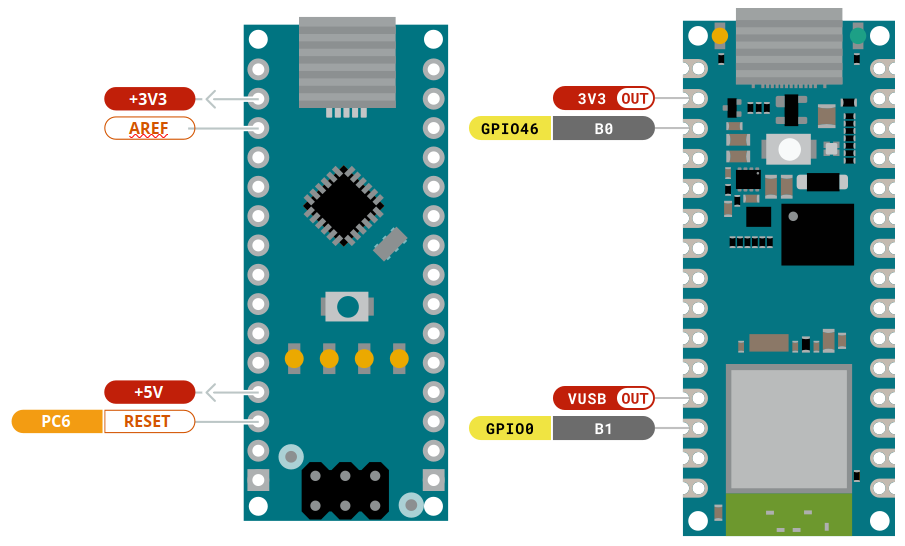
\includegraphics[width=\textwidth, center]{img/nano-differences-m.png}
    \caption{Hervorgehobene Unterschiede in der Pinbelegung zwischen Arduino und ESP32 nano}
    \label{fig:nano_boards}
\end{figure}

Zwischen den Boards zeigen sich die folgenden Unterschiede.
\begin{itemize}
    \item Pin 3 von \texttt{AREF} zu \texttt{GPIO46} und \texttt{Boot0}.
    \item Pin 12 von \texttt{+5V} zu \texttt{VUSB} oder \texttt{VBUS}.
    \item Pin 13 von \texttt{RESET} zu \texttt{GPIO0} und \texttt{Boot1}.
\end{itemize}

Der Pin 3 von \texttt{AREF} ist unproblematisch, 
da er zu einem ungenutzten I/O Interface führt.

Pin 12 erfordert Beachtung,, weil der \texttt{VBUS} im Vergleich zu \texttt{+5V} als
direkte Verbindung von der Versorgung aus der USB Schnittstelle bedacht wurde und 
dadurch vom Board nicht weiter geregelt wird. Deswegen wird empfohlen, 
den VBUS nicht mit anderen Pins am Nano kurzzuschließen. 
Wenn aber der ESP32 über den VIN Pin versorgt ist, 
wird der Pin deaktiviert und sollte keine 5V von der USB Schnittstelle liefern können. 
% Weiteres verhalten darüber hinaus ist nicht dokumentiert.
% Mehr dazu und der anderen Betriebsspannung ist in Abschnitt \ref{subsec:problem_betriebsspannungen} zu finden.

Pin 13 sollte keine Probleme machen, da er zu einem offenen Schalter geht,
der ursprünglich den \texttt{RESET} Pin betätigt hätte und sonst offen liegt.
%
Beim ESP32 würde der Schalter dafür sorgen, 
dass entweder zum Boot Mode gewechselt werden kann, 
oder zu gewöhnliche Operationen mit \texttt{GPIO0}.
%
Jedoch kam es zu Störungen an diesem Pin, 
weshalb die Verbindung getrennt wurde,
in dem der Pin am Header ausgebaut wurde.

\subsection{Linux Modifikationen}
\initials{JS}
Es kam das Problem auf, 
dass die lokale IP-Suche auf Linux-Systemen nicht funktioniert.
%
Dies lag daran,
dass die vorherige Variante mithilfe des Domain-Namens die lokale IP-Adresse findet.
%
In Linux wird jedoch eine andere Adresse zurückgeliefert, 
und zwar die Loopback-Adresse \texttt{127.0.1.1}.
%
Diese Adresse wird verwendet,
um dem \texttt{host\_name} eine Adresse zuzuweisen,
im Falle, dass kein Netzwerk vorhanden ist.
%
Ansonsten kann eine permanente IP-Adresse hier zugewiesen werden.
% https://askubuntu.com/questions/754213
% /what-is-difference-between-localhost-address-127-0-0-1-and-127-0-1-1

Als Lösung öffnet das Programm temporär einen Socket 
und findet mit diesem die lokale IP-Adresse,
wodurch es plattformunabhängig wird.
\begin{lstlisting}[language=python, gobble=4]
    import socket

    def get_local_ip():
    """
    opens a temporary socket connection and retrieves the local IP
    """
    s = socket.socket(socket.AF_INET, socket.SOCK_DGRAM)
    try:
        # doesn't even have to be reachable
        s.connect(('10.255.255.255', 1))
        IP = str(s.getsockname()[0])
    except Exception as b:
        print("error at figuring out local ip")
        print(b)
        exit
    finally:
        s.close()
    return IP
\end{lstlisting}

\subsection{Potenzielles blockierendes Verhalten}
\initials{JS}
% bot_handler und server nicht separat gestartet werden.
Obwohl die Kommunikation in zwei Teile aufgeteilt ist, 
mit Bot-Handler und Server, 
werden sie zu diesem Zeitpunkt gemeinsam gestartet.
%
Dies führt zu der ungewollten Konsequenz, dass,
falls der Bot-Handler sich frühzeitig oder ungewollt beendet,
dieser nicht neu gestartet wird, bis sich ein neuer Client verbindet.
% 
Da jedoch für diese Diplomarbeit zu erwarten ist, 
dass die Bots stets zur Verfügung stehen sollten,
wird der Prozess bei einer geschlossenen Verbindung für eine gewisse Zeit pausiert,
bevor ein neuer Verbindungsversuch gestartet wird.
%
In den nächsten Iterationen sollten jedoch 
die zwei Aufträge unabhängig gestartet werden können, 
um zu vermeiden,
dass die ganze Kommunikation neu gestartet werden muss.

\subsection{Protobuf Generierung}
\initials{JS}
% siehe server/README.md
% verlege zu Backend probleme?
Während der Migration vom Vorentwicklungsordner, 
wurde für eine gewisse Zeit in einem Testordner experimentiert.
%
Dies führte dazu, dass der generierte Protobuf-Code nicht funktionierte,
da der Wrapper nicht über den Unterordner Standort \text{protobuf} 
der weiteren Protobuf-Dateien ``informiert'' wurde.
Dies war der Fall da das Kompilieren der Protobuf-Dateien für Python unabhängig vom Standort
der Python-Umgebung geschieht, 
wodurch die Importe im generierten \text{wrapper\_pb2.py}
mit dem Ordner vorangestellt werden müssen.

\begin{lstlisting}[language=python, gobble=4]
    import protobuf.move_cmd_pb2 as move__cmd__pb2
    import protobuf.led_cmd_pb2 as led__cmd__pb2
    import protobuf.lidar_data_pb2 as lidar__data__pb2
    import protobuf.encoder_data_pb2 as encoder__data__pb2
    import protobuf.imu_data_pb2 as imu__data__pb2
\end{lstlisting}
